\chapter{Theoretical background}
\label{ch:theoreticalbackground}
This chapter defines the core concepts of the research. These concepts are the \gls{ps}, \acrlong{ea}, and \gls{antifragile}. The concepts make use or contain the concept system. This chapter will also define the concept of system.

\section{Antifragile}
\label{sec:tbantifragile}




\section{System}
\label{sec:tbsystem}

\subsection{The boundary of a system}
To what extend does something belong to a system. As defined by \textcite[p. 182-183]{Gharajedaghi2011}, the boundary of a system consists of all the variables that can be sufficiently influenced or controlled by participating actors. The variables that can not be influenced or controlled but impact the viability of the system are part of the context.

\subsection{System of Systems}





\subsection{The public sector as a System of Systems}
\label{sub:tbpssystemofsystems}

\section{Public sector}
\label{sec:tbpublicsector}

As talked about in chapter \nameref{ch:introduction} the \gls{ps} is generally divided into three levels \parencite{PrivacySense2016}.

\begin{itemize}
	\item{\textbf{The national government,} such as the military, the tax authority, and homeland affairs.}
	\item{\textbf{The regional government,} such as the provinces, the police, and water management.}
	\item{\textbf{The local government,} such as the municipalities, the social services, and the local tax offices.}
\end{itemize}

\begin{figure}[H]
	\centering
	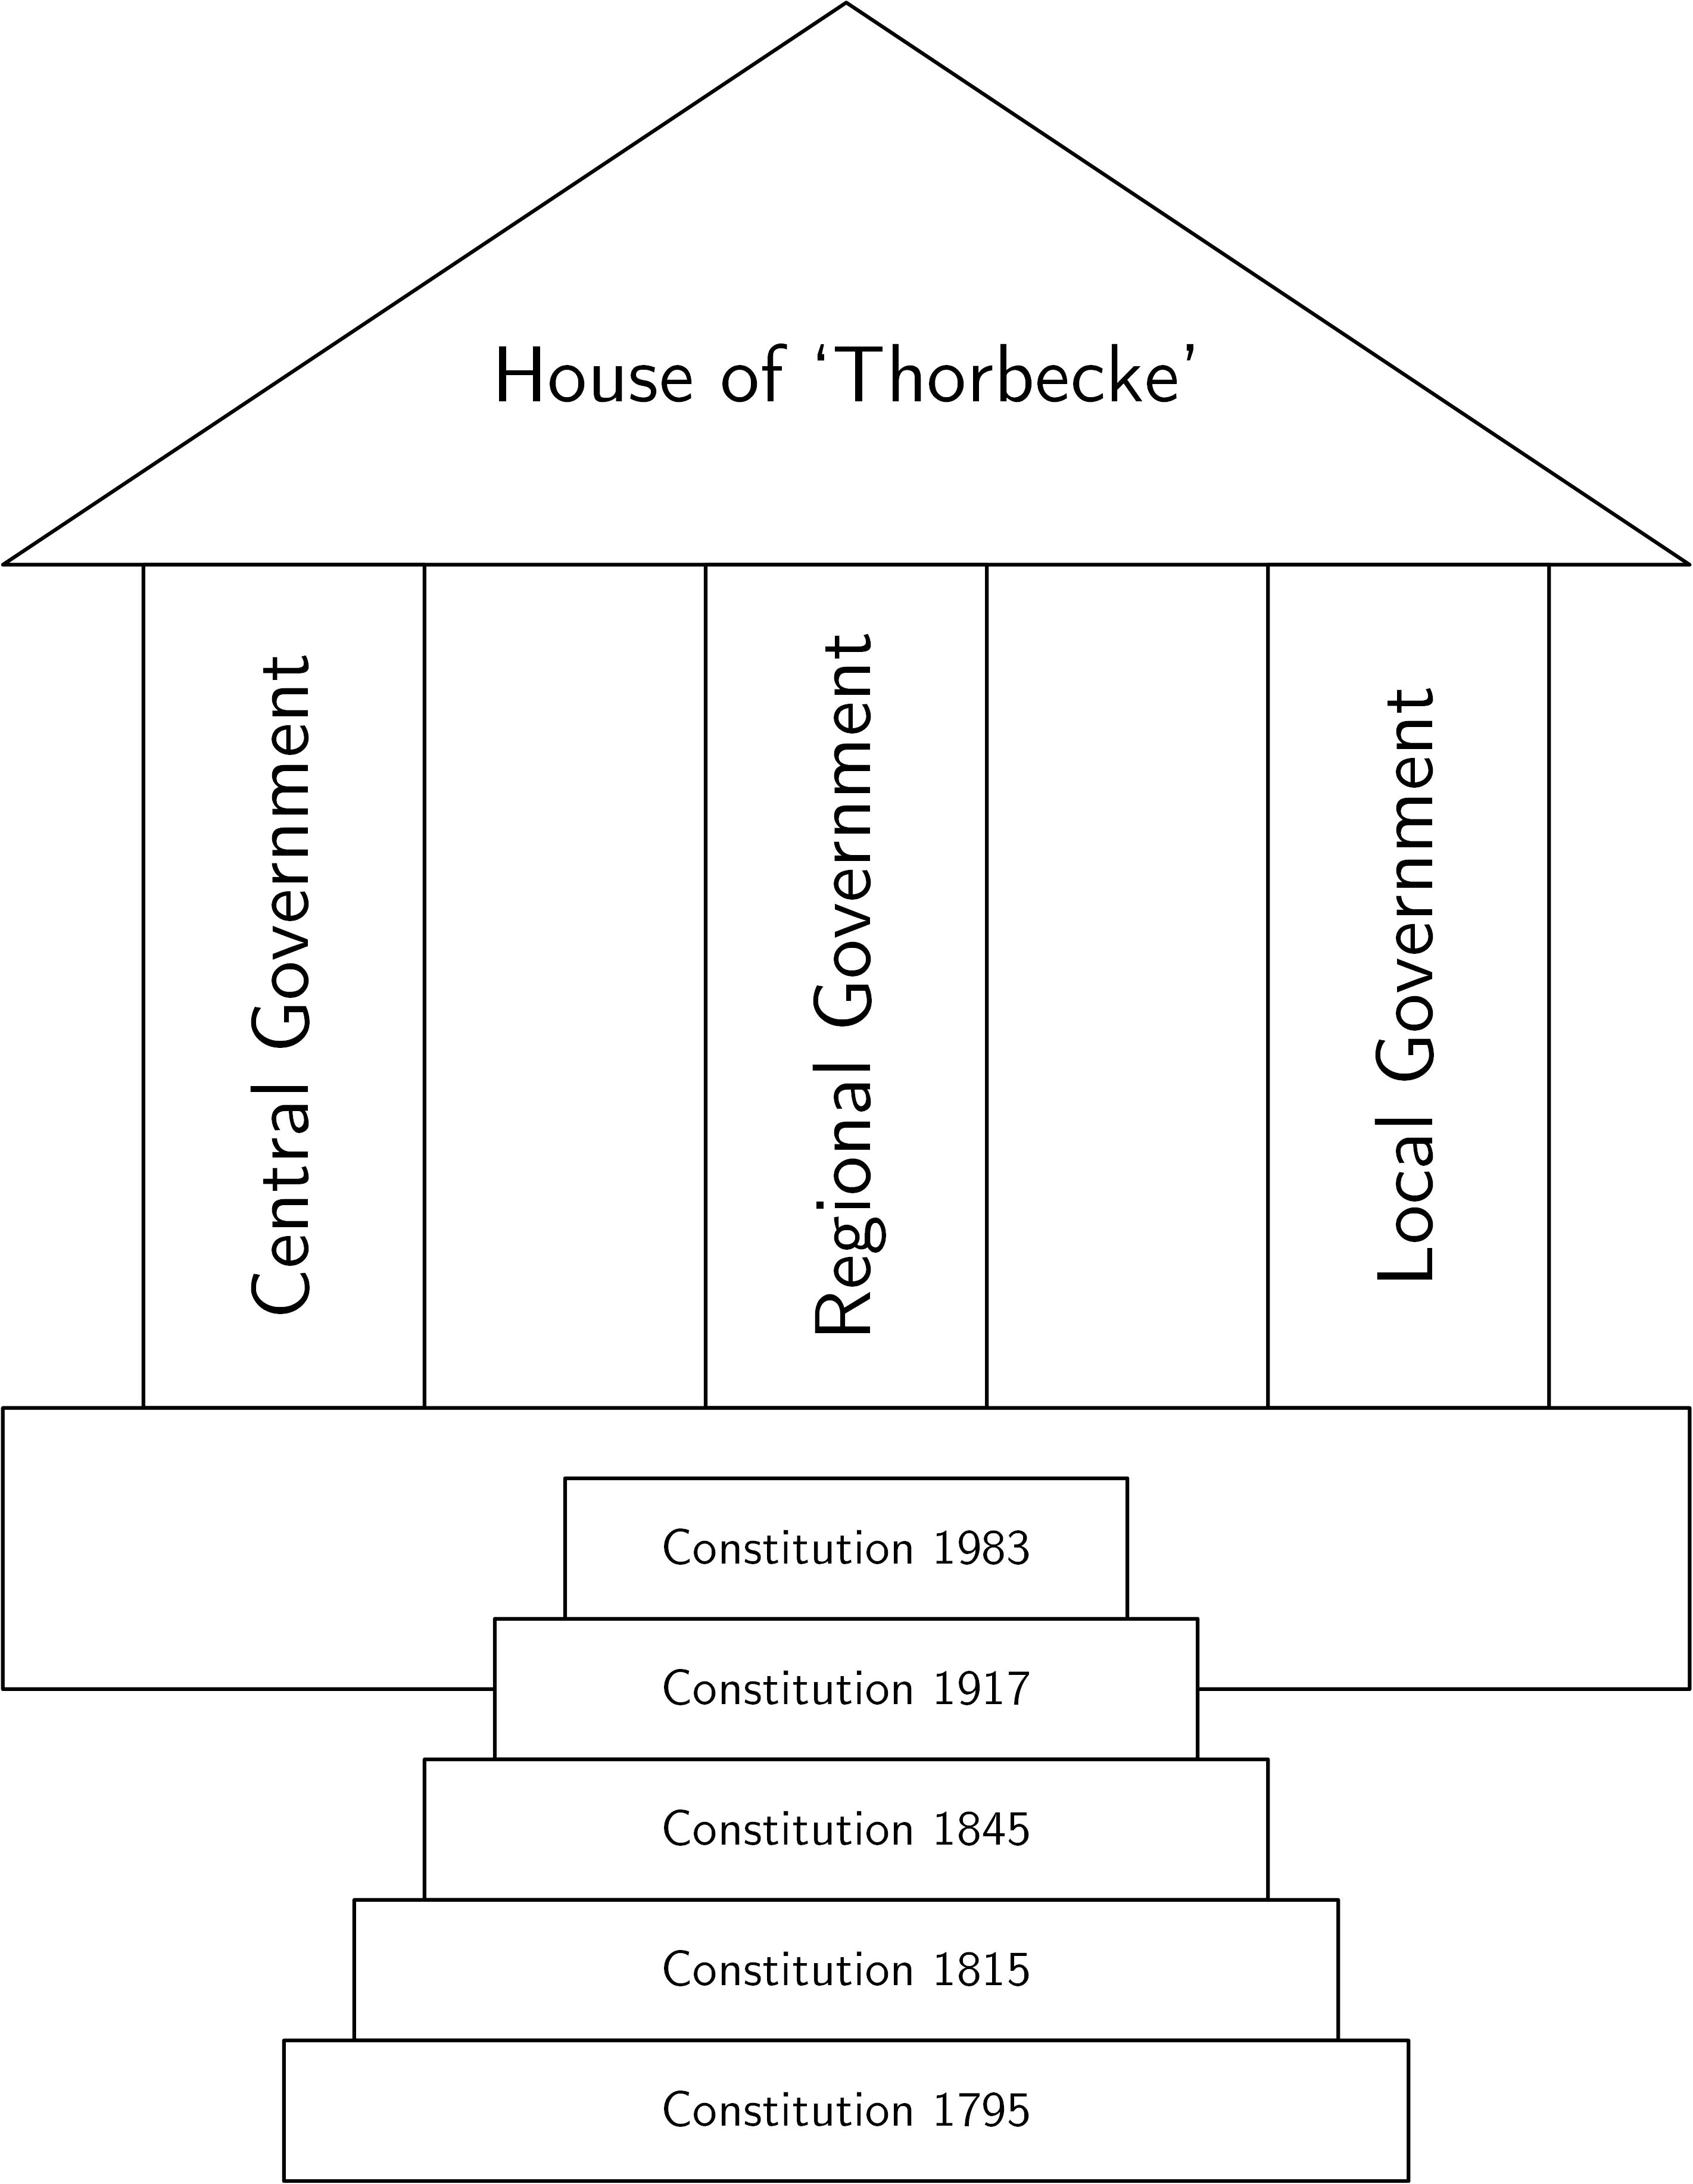
\includegraphics[width=0.4\linewidth]{images/thorbecke}
	\caption[The House of 'Thorbecke']{The House of 'Thorbecke'}
	\label{fig:houseofthorbecke}
\end{figure}


I will focus this research on the public sector level local government of the Netherlands. In \cref{ch:discussion} I will discuss the applicability on non Dutch public sectors.



\subsection{Collaboration between public and private sector}

More often the public sector is partnering with a privatly held organisation to create a public-private partnership or \acrfull{jv}. These hybrid organisations work together to deliver a service or business venture to a community jointly. Through outsourcing, public sector organisations will often engage the private sector to deliver goods and services to their citizens. 

\begin{figure}[H]
	\centering
	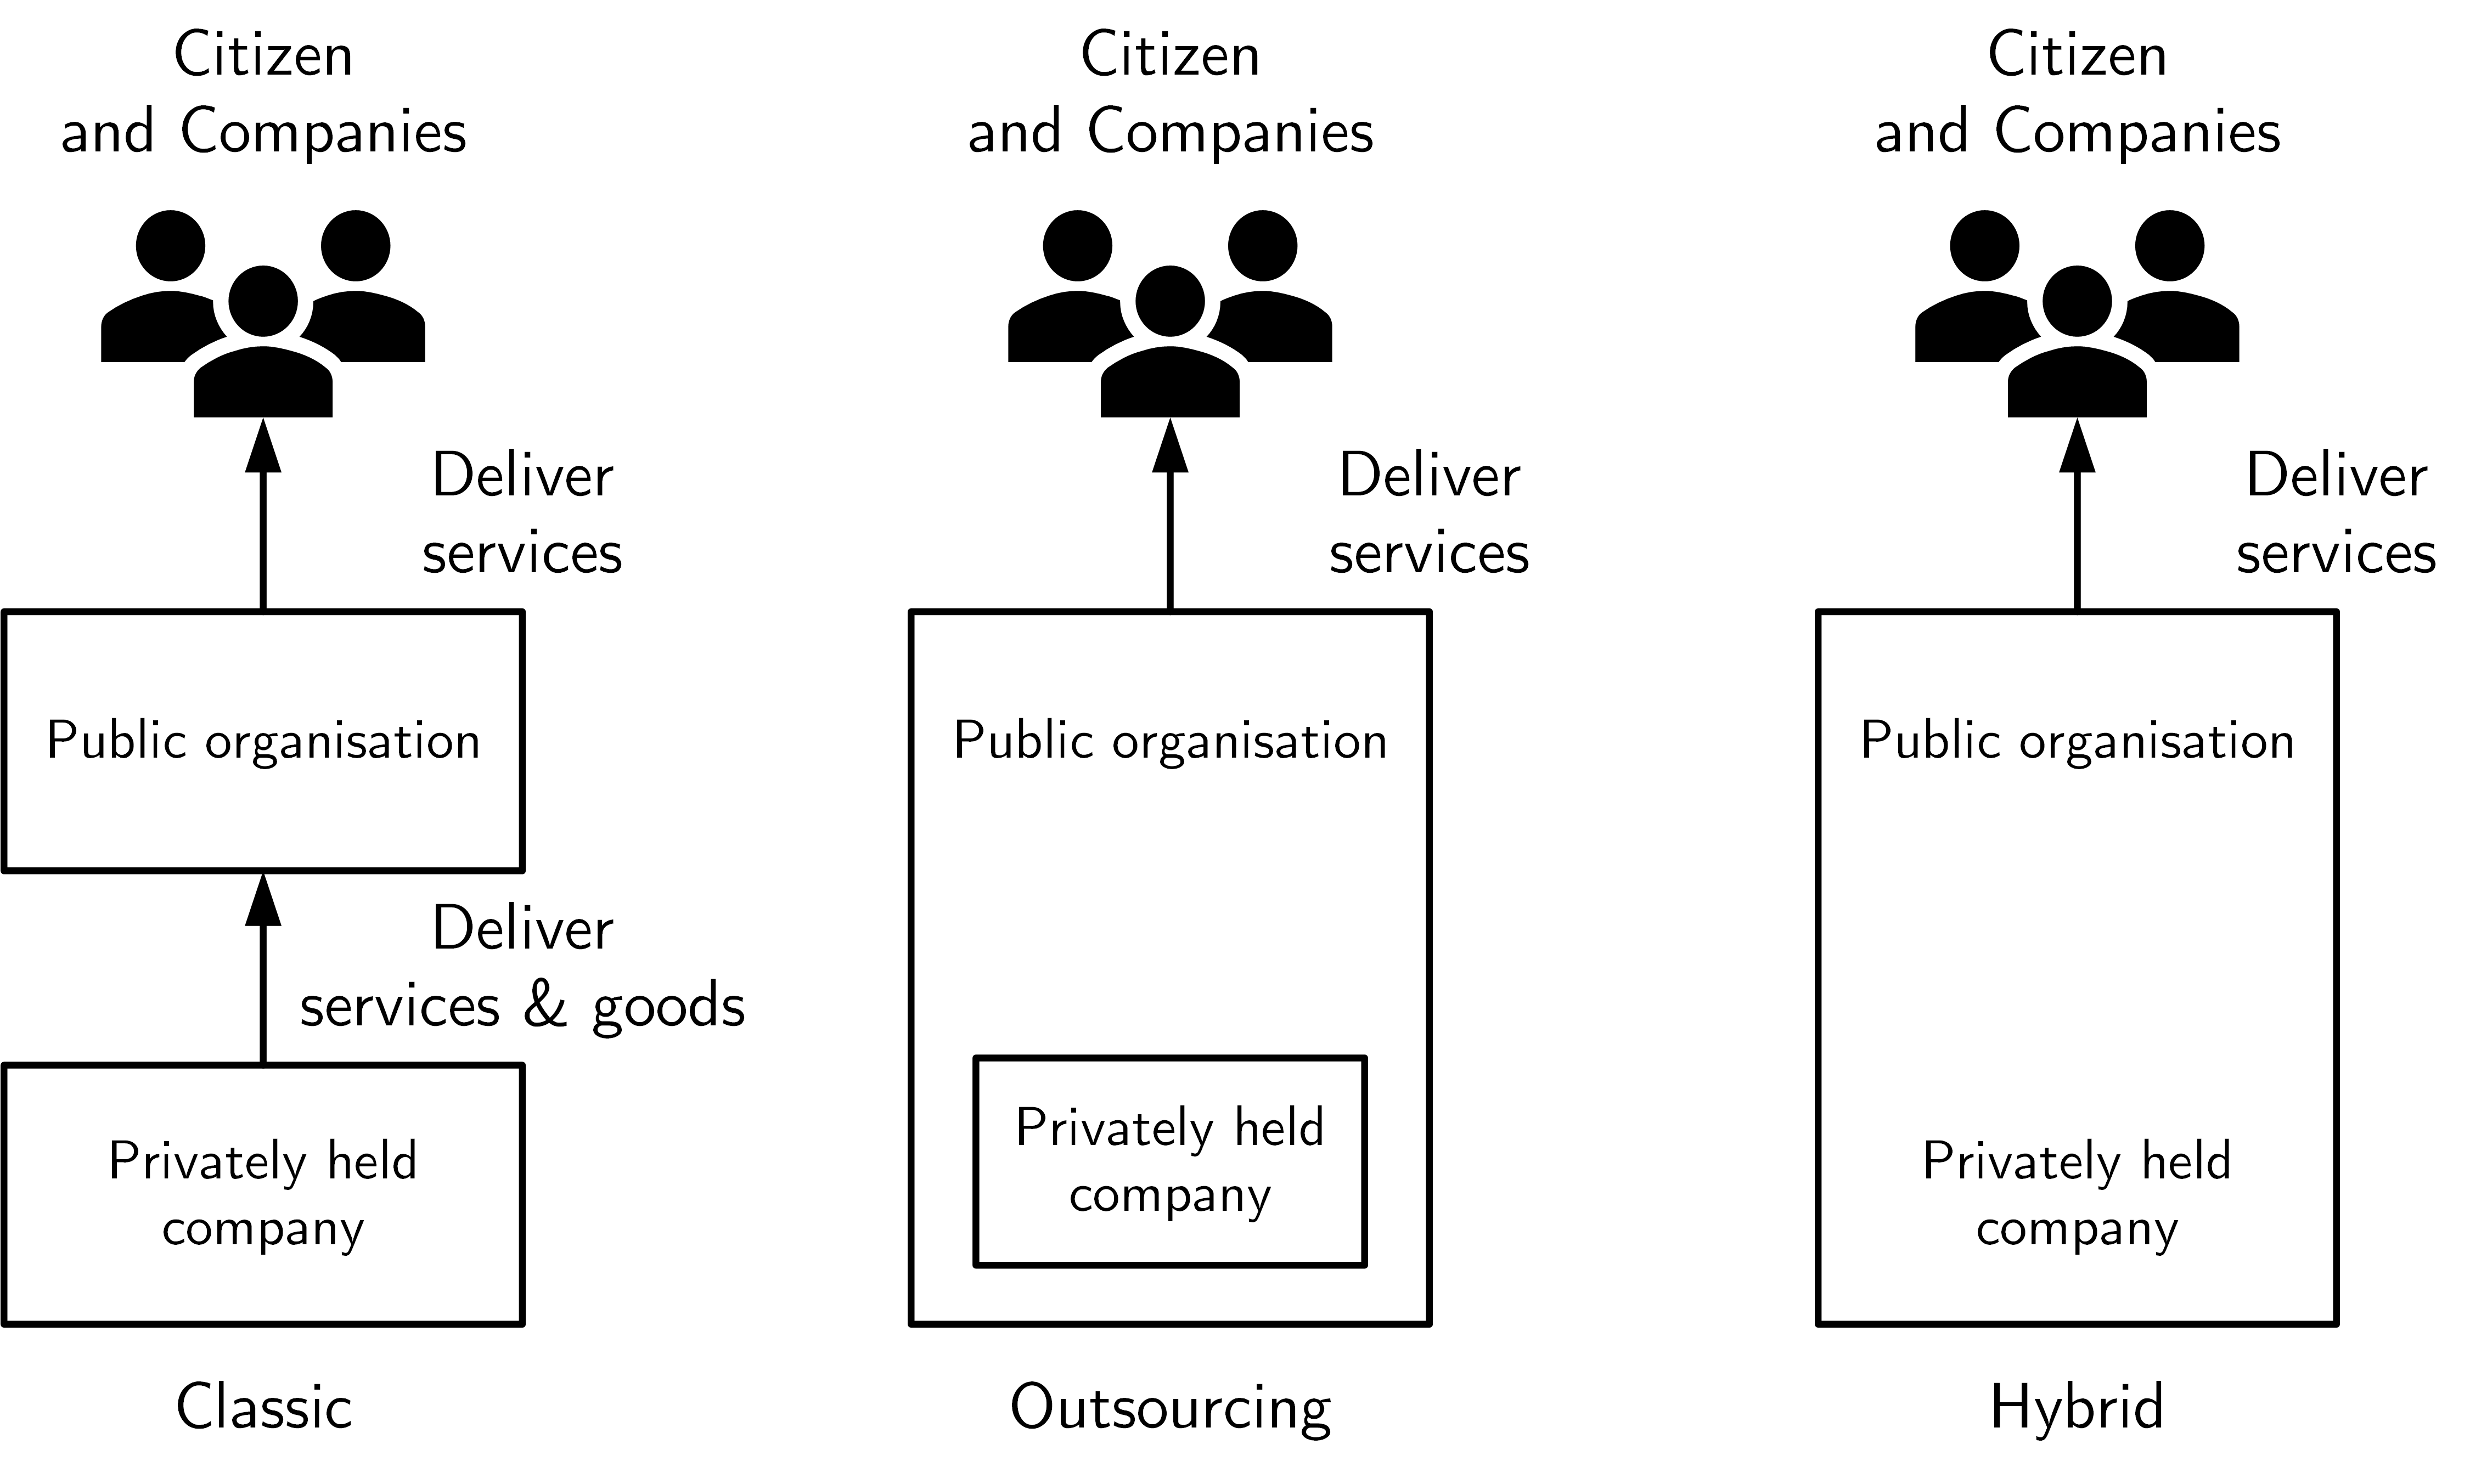
\includegraphics[width=0.7\linewidth]{images/publicsector3modelsofcolaboration}
	\caption[Public sector collaboration models]{Public sector collaboration models}
	\label{fig:publicsector3modelsofcolaboration}
\end{figure}

I argue that, in the hybrid model, the definition of the public sector is not correct anymore. The part of a private company that is a part of a hybrid collaboration, in a \gls{jv}, with the public sector should be part of the public sector system.

\subsection{Differences with the Private Sector Market}
\label{sub:tbdifferenceprivatesector}



The core values are different in the public sector than that of the private sector. The top five private sector core values are profitability, accountability, expertise, reliability, and effectiveness. The top five public sector core values are accountability, effectiveness, incorruptibility, reliability, and lawfulness. \parencite{Wal2008} Profitability is only a value for the private sector, and it does not exist as a value for the public sector.  The public sector demands or even initiates changes without noticing the needed investments to execute these changes by the private sector.

\section{Enterprise Architecture}
\label{sec:tbenterprisearchitecture}
There are various definitions of \acrlong{ea}, and there is no agreement on them. The various definitions are not always complimentary, and sometimes they are in opposite \parencite{Lapalme2012,SaintLouis2019,Hoogervorst2009}. 

\textcite{White2018} states that the organisations business requirements guide \acrshort{ea}. \acrshort{ea} helps layout how information, business and technology flow together. While \textcite{Gartner} states that Enterprise Architecture is a discipline for proactively and holistically leading enterprise responses to disruptive forces by identifying and analysing the execution of change toward desired business vision and outcomes. \acrshort{ea} delivers value by presenting business and IT leaders with signature-ready recommendations for adjusting policies and projects to achieve targeted business outcomes that capitalise on relevant business disruptions. \textcite[p. 9]{Ross2014} defines \acrshort{ea} as the organising logic for business processes and IT infrastructure, reflecting the integration and standardisation requirements of the company’s operating model. The \acrshort{ea} provides a long-term view of a company’s processes, systems, and technologies so that individual projects can build capabilities and not just fulfil immediate needs. Following \textcite[p. 4]{Graves2009} \acrfull{ea} is the discipline through which an enterprise can identify, develop and manage its knowledge of its purpose, its structure and itself. Some of that knowledge will be about IT, but it will also need to include many other concerns like (e.g.): ''Business, Process, Secyrity, Data, Application, and technology-infrastructure architecture as well as organisational structures, performance management, and  business continuity \& resilience planning \parencite[p. 4]{Graves2009}.''

By using the \acrshort{ea} discipline \acrshort{ea} provides decision-support for direction and change at any level of the enterprise \parencite[p. 4]{Graves2009}, e.g.: ''The choices in the journey of an enterprise for an executive, the preffered technologies of process models for new developments for programme and portfolio management, as well plan as planning when to decomission, change or replace systems \parencite[p. 4]{Graves2009}.''

Mature \acrshort{ea} can map interdependencies across almost every aspect of the enterprise \parencite[p. 5]{Graves2009}. A well defined and maintained \acrshort{ea} is proven to be a critical factor in an organisation's agility, effectiveness and ability to respond to risk, opportunity and change \parencite{Ross2014}.  \textcite[p. 5]{Graves2009} states somewhat the same with that \acrshort{ea} assists in managing changes imposed on the organisation from outside, by the market, by regulations, or at an operations level, by system failures, environmental incidents or customer complaints.

When I consider, following \cref{sub:tbpssystemofsystems}, the \gls{ps} as a \acrfull{sos} the definitions of \acrshort{ea} of \textcite{Gartner,Graves2009} do align with \acrshort{sos}. If I take into account that \textcite{Graves2009} is one of the authors of the third school of thought, see for more details \cref{sub:eaapproaches}, I will use the definition of \citeauthor{Graves2009} for this research.

\subsection{Approaches of Enterprise Architecture}
\label{sub:eaapproaches}
There are several approaches to the practice of \acrshort{ea}. \textcite{Ylinen2018,Ylinen2020,Kotusev2015,Lapalme2012} conducted research to these approaches. \textcite{Ylinen2018,Ylinen2020} found an approach in which they can distinguish two groups of \acrshort{ea} experts. A modelling-focused group forms a comprehensive view of an organisation and a development-focused group using \acrshort{ea} for organisational development. 

\textcite{Kotusev2015} distinguished three approaches. These three approaches are the traditional, the \acrfull{mit}, and the \acrfull{dya} approach. The traditional approach, initially presented by \textcite{Spewak1993}, to \acrfull{eam}, can be generally described as a four-step sequential process: -1- document the current (as-is, baseline) state, -2- develop the desired future (to-be, target) state, -3- develop the transition plan to migrate from the current to the future state, -4- implement the plan and then repeat the whole process all over again \parencite[p. 4071]{Kotusev2015}. The \acrshort{mit}, developed by \textcite{Ross2014}, approach advocates the development of a core diagram reflecting a long-term enterprise-level architectural vision. This abstract architectural vision should be later translated into concrete project-level decisions through IT governance mechanisms involving business and IT managers on different organizational levels \parencite[p. 4072]{Kotusev2015}. \acrfull{dya}, initially presented by \textcite{Wagter2005}, advocates “just enough, just in time” architecture, no \acrshort{ea} is designed until there is a need for it. \acrshort{eam} activities in the \acrshort{dya} approach are triggered by concrete business initiatives appearing in the process of strategic dialogue. As a response to a new business initiative, architectural services update \acrshort{ea} if necessary and prepare a project-start architecture for a new project in order to ensure that this new project fits nicely into existing \acrshort{ea} and larger picture \parencite[p. 4072]{Kotusev2015}. 

\textcite{Lapalme2012} is using a different approach. He defined three schools of thought on \acrshort{ea}. The first school is about Enterprise IT Architecting. The first school is about aligning an enterprise's IT assets to execute business strategy effectively and various operations using the proper IT capabilities  \parencite[p. 38]{Lapalme2012}. With the first school of thought, \acrshort{ea} is the glue between business and IT. The second school of thought is Enterprise Integrating. This school is about designing all facets of the enterprise. The goal is to execute the enterprise's strategy by maximizing the overall coherency between all of its facets. This school is grounded in systems thinking. This school approaches enterprise design holistically or systemically \parencite[p. 40]{Lapalme2012}. For the second school, \acrshort{ea} is the link between strategy and execution. 

The last school of thought is \acrfull{eea}. This school, \acrshort{ea} is about fostering organisational learning by designing all facets of the enterprise, including its relationship to its environment, to enable innovation and system-in-environment adaptation. Creating the enterprise strategy and designing the organisation are top priorities. Like the enterprise integration school, this school is concerned with contradictions, not just within the organisation. The third school looks for incoherence in the bidirectional relationship between the enterprise and its environment \parencite[p. 40-41]{Lapalme2012}. For the third school of thought, \acrshort{ea} is the means for organisational innovation and sustainability. For detailed properties of the schools of thought, see Appendix '\nameref{app:easchoolsproperties}'.

\textcite{Lapalme2012} defined the scope of \acrshort{eea} ''the enterprise in its environment, including not only the enterprise but also its environment and the bidirectional relationship and transactions between the enterprise and its environment'' with the purpose to ''help the organization innovate and adapt by designing the various enterprise facets to maximize organizational learning throughout the enterprise.'' As \textcite{Botjes2020} concluded with his \acrshort{eaal} model the attribute learning organisation is of importance for being \gls{resilient} or \gls{antifragile}. If the learning organisation is one of the conditions to be \gls{antifragile} the practice of \acrshort{ea} should be of the school of \acrshort{eea}. 



